%%「論文」,「レター」,「レター(C分冊)」,「技術研究報告」などのテンプレート
%% 1. 「論文」
%% v1.6 [2009/11/03]
\documentclass{ieicej}
%\documentclass[invited]{ieicej} % 招待論文
%\documentclass[comment]{ieicej} % 解説論文

\usepackage{cleveref}
\usepackage{graphicx}


%\usepackage{latexsym}
%\usepackage[fleqn]{amsmath}
%\usepackage[psamsfonts]{amssymb}

\setcounter{page}{1}

% \field{}
\jtitle{}
\etitle{Performance Evaluation of Docker Image Transfer toward Optimal Containers Deployment}

\authorlist{
\authorentry{}{Kai LIU}{1}
\authorentry{}{Kento AIDA}{2}
\authorentry{}{Shigetoshi YOKOYAMA}{2}
\authorentry{}{Yoshinobu MASATANI}{2}% <= 記述しないとエラーになります
 %\authorentry{和文著者名}{英文著者名}{所属ラベル}
 %\authorentry[メールアドレス]{和文著者名}{英文著者名}{所属ラベル}
 %\authorentry{和文著者名}{英文著者名}{所属ラベル}[現在の所属ラベル]
}
\affiliate[1]{}{The Graduate University for Advanced Studies}
\affiliate[2]{}{National Institute of Informatics}
%\affiliate[所属ラベル]{和文所属}{英文所属}
% \paffiliate[1]{SOKENDAI (The Graduate University for Advanced Studies)}
% \paffiliate[現在の所属ラベル]{和文所属}

\usepackage{cite}
\usepackage{url}

\begin{document}

% \begin{abstract}
%和文あらまし 500字以内
% \end{abstract}
% \begin{keyword}
%和文キーワード 4~5語
% \end{keyword}

\begin{eabstract}
Abstract  Nowadays, how to utilize clouds to perform big data analysis is becoming a practical issue. The rise of container technology such as Docker simplifies the process of deploying big data application in clouds. However, the resource selection problem challenges users to maximize performance. In this paper, we evaluate Docker image transfer time as the first step to tackle optimal resource selection problem.
\end{eabstract}
\begin{ekeyword}
Big Data, Cloud Computing, Docker
\end{ekeyword}
\maketitle

\section{Introduction}
With the rapid growth of data amount around the world, traditional compute platforms can hardly fulfill the requirements of big data storage and analysis. Cloud platforms, such as Amazon Web Services \cite{amazon2015aws}, Microsoft Azure \cite{microsoft2015azure} and Google Cloud Platform \cite{google2015cloud}, are expected to be promising big data processing platforms as they can provide powerful, elastic and economical storage and computation ability. In addition, both IaaS, PaaS and SaaS can be adopted to implement big data analytics in the cloud \cite{domenico2013clouds}. In this paper, we focus on utilizing IaaS to process big data using applications built by users.


One of the biggest challenges to utilize clouds for big data processing is how to select resources to optimize the overall performance. In this context, resources mean data to be processed, applications processing data and clouds for running big data processing application. To initiate a big data processing on clouds, we need to transfer data to clouds, deploy big data processing applications on clouds and then run the applications. However, data, applications and clouds are distributed in different locations. The data can be stored in private infrastructures, public storage clouds or other data warehouses. Applications, which are packaged in Docker \cite{docker2015} images according to our assumption, can exist in public Docker registries, private Docker registries or local platforms. In addition, cloud platforms also locate in different geographical regions. Therefore, all resources should be carefully selected to minimize the total processing time, which includes the time of transferring data, deploying applications and processing data.


For big data analysis, transferring data and processing data will introduce significant overhead. A lot of researches studying data transfer and data processing have been conducted. However, the problem of deploying applications attracts less attention. As a matter of fact, deploying a big data analysis application in clouds is also nontrivial even for experienced programmers, not to mention data analysis users who possess limited computer skills. The development of Linux container technology like Docker, which is able to package applications into lightweight images, has changed the way of deploying application greatly. Theoretically, we can package any applications into Docker images, transfer these images to any cloud platform and build the big data analysis environment immediately. Furthermore, Cloud providers, e.g. Amazon Web Services, Google Cloud Platform, currently support Docker on their platforms \cite{amazon2015container,google2015container}. This can also help people to utilize multiple clouds without worry about vendor lock-in problem. In this paper, we assume that big data processing applications are packaged in Docker images. Thus, the Docker image transfer time accounts for an important part of the whole data analysis process, especially for applications consisting of lots of short running tasks.


Docker, as the most successful and popular container tool, has gained a lot of attractions from both industry and academia. Recent researches \cite{felter2014updated,tang2014performance,morabito2015hypervisors} find that Docker shows better performance than the virtual machine technology. Other researchers concentrate on using Docker for packaging applications to solve the ``dependency hell'' problem \cite{gerlach2014skyport,zheng2015integrating,boettiger2015introduction,tazro2015read}. To the best of our knowledge, the performance of Docker image transfer has not been discussed.

In this paper, we present the performance evaluation results of Docker image transfer over LAN/WAN settings. We launched some benchmarks to transfer Docker images from the same source node to three different destination nodes. NII Tokyo node is the source node and destination nodes are NII Chiba, EC2 Tokyo and EC2 Virginia Nodes. NII Chiba Node and the source node are located in geographically different sites but connected through the same VLAN of our institute, while EC2 Tokyo node and EC2 Virginia Node are connected with the source node through WAN. In addition, only EC2 Virginia Node resides in US and other nodes are located in Japan. The experimental results reveal that Docker image transfer time shows strong linear relationship with the image size. While Docker registry 2.0.1 showed better performance and reliability than Docker registry 0.9.1, we observed the performance instability we ran the Docker registry 2.0.1 on EC2 nodes. In addition, running Docker registry on local or remote nodes present similar performance.

The remainder of the paper is organized as follows. Section 2 introduces Docker and related work, providing necessary background to understanding the rest of the paper. Section 3 provides the tentative scenario of deploying big data analysis application on cloud platforms. Section 4 shows the experimental setup while section 5 presents the experiment results. Finally, we conclude the work presented in this paper in Section 6.

\section{Background and related work}
\subsection{Docker}
Compared to virtual machine technology, the Linux container technology is a more lightweight virtualization technology. Multiple containers running on the same host share the same OS with the host while coexisting virtual machines run their independent OSs. Therefore, the container technology can provide near native performance, higher density and faster start/stop time. Modern linux kernel features, such as Namespaces \cite{michael2013namespaces} and Cgroups \cite{paul2015cgroups}, are building blocks for container technology. Namespaces are the key to isolate containers with the host and other containers, and Cgroups can help containers control the usage of resources like CPU and memory. Although the container technology has existed for over a decade, only recently have it gained increasing attraction from both industry and academia. Due to some advanced features described later, Docker is becoming a standard Linux container tool rapidly.

Docker, the most popular and successful container tool, outperforms other container pioneers like OpenVZ \cite{openvz2015}, Linux VServer \cite{vserver2015} and Warden \cite{warden2015}. By using Docker, we can easily create, stop, restart and delete containers. This great user friendliness contributes a lot for thesuccess of Docker. The ability to package an application and its dependencies into a lightweight Docker image is another advanced feature of Docker. Therefore, we can download Docker images and run the application in any Docker enabled host without worry about laborious installation processes. This also helps us a lot to quickly deploy big data applications in clouds.


\subsection{Related Work}
The performances of Docker have been discussed in literatures. By running a suite of workloads that stress the CPU, memory, storage and networking resources, the research group in IBM found that the performances on Docker were in equal or better than those on KVM in almost all cases \cite{felter2014updated}.  Tang \cite{tang2014performance} compared KVM and several lightweight virtualization techniques, including Lmctfy, ZeroVM and Docker. The result showed that Docker had better performance, faster deployment and weaker isolation. Morabito \cite{morabito2015hypervisors} presented a detailed performance evaluation of KVM, Docker, LXC and OSv. Unsurprisingly, the performance overhead of Docker could be considered almost negligible.


Other researchers are interested in using Docker to package applications into Docker images, making software installation more convenient. For example, Skyport \cite{gerlach2014skyport} is the extension of the data analysis platform---AWE/Shock and it greatly reduces the heavy burden of providing the environment to execute complex workflows. Zheng \cite{zheng2015integrating} proposed to utilize Docker to deliver workflow execution environment and focused on how to best integrate Docker into workflow system. Boettiger \cite{boettiger2015introduction} claimed that Docker was a promising tool to address the challenges of scientific reproducibility. Ohta \cite{tazro2015read} discussed a platform of reproducible computer experiments using Docker for genome sequencing applications.

\section{Tentative user scenario}


\begin{figure}
  \begin{center}
  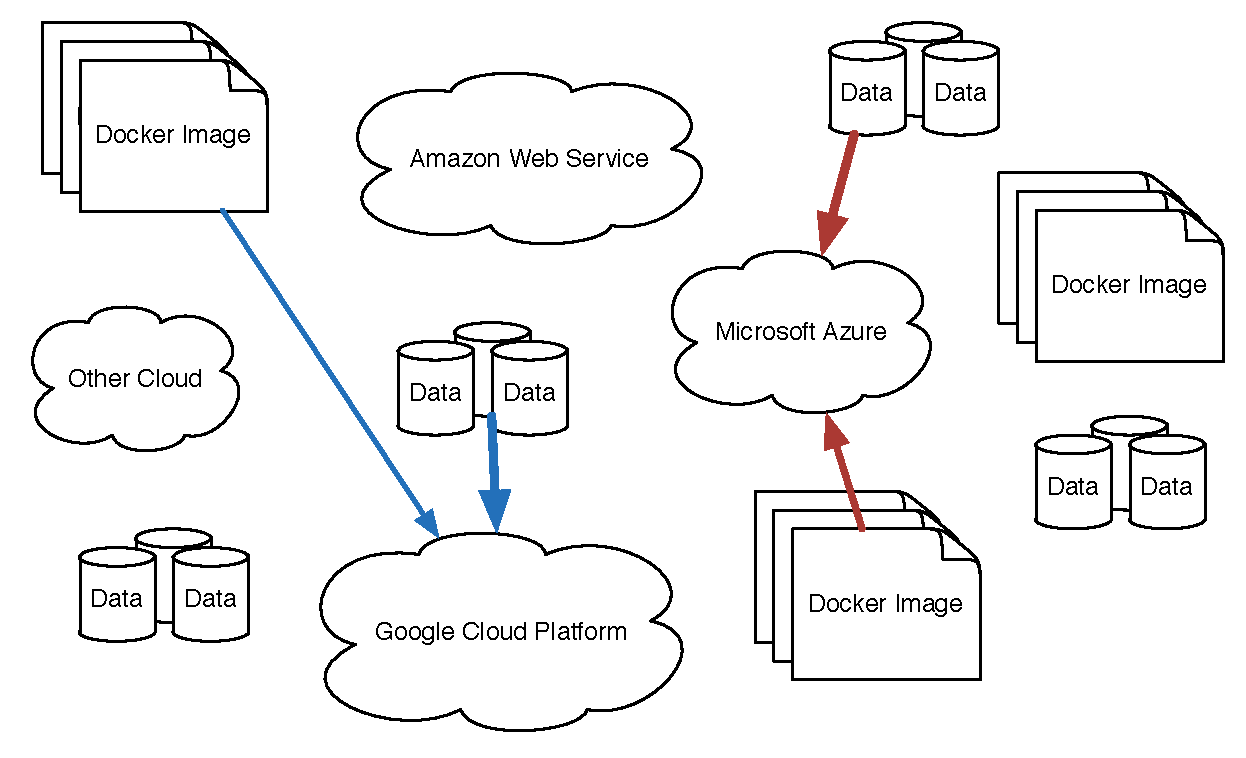
\includegraphics[width=0.8\textwidth,natwidth=1000,natheight=450]{1_Tentative_user_scenario.pdf}
  \end{center}
  \caption{Tentative user scenario}
  \label{tentative_user_scenario}
\end{figure}


\begin{table*}[t]
  \begin{center}
% \begin{figure*}[t]
  \begin{tabular}{| c | c | c | c | c |}
  \hline
    Nodes   & NII Tokyo    & NII Chiba        & EC2(m3.2xlarge) Tokyo    & EC2(m3.2xlarge) Virginia \\
  \hline
    Memory  & 31GB         &  94GB            & 29GB                     &  29GB \\
  \hline
    Disk    & 932GB        &  2.5TB           & 8G                       &  8G \\
  \hline
    OS      & Ubuntu 14.04 &  Ubuntu 12.04    & Ubuntu 14.04             & Ubuntu 14.04 \\
  \hline
  \end{tabular}
  \caption{Benchmark nodes information}
  \label{bench_nodes_info}
  \end{center}
% \end{figure*}
\end{table*}

Figure 1 illustrates a tentative user scenario of Docker image transfer discussed in this paper. In the scenario, the user runs a data processing application, where data and Docker images are distributed in different locations on the Internet and the user has options of cloud platforms to run the user's application. To efficiently harness cloud platforms for the user's application, it is very important to select optimal set of resources to maximize the overall application performance. Therefore, evaluating the Docker image transfer time is the first step to develop resource selection strategy.


\section{Experimental setup}
\subsection{Tested}
To evaluate Docker image transfer time, we ran benchmarks to transfer Docker images from the same source node (NII Tokyo Node) to three different destination nodes (NII Chiba, EC2 Tokyo and EC2 Virginia Nodes).
NII Chiba Node and the source node are located in geographically different sites but connected through the same VLAN of our institute, while EC2 Tokyo node and EC2 Virginia Node are connected with the source node through WAN.
In addition, only EC2 Virginia Node resides in US and other nodes are in Japan.
Detailed information about these nodes can be found in \cref{bench_nodes_info}.
All four nodes run Docker 1.6.2. To transfer a Docker image from the source node to the destination node, we push the image to the Docker registry first, and then pull the image from the Docker registry.
We refer to this method as the pushpull method.
The Docker registry ran in Docker container instead of on the host node so that we can more flexibly configure the experimental setup.

\subsection{Benchmarks}
We selected a set of Docker images presented in \cref{bench_img_l} for our benchmark. For each benchmark setting, we evaluated the transfer time of 31 different Docker images with sizes ranging from 1.3MB to 1.3GB.
\cref{bench_img_l} shows the detailed information about these images and all images can be obtained from Docker Hub \cite{dockerhub2015}.
These images have different image sizes and each image consists of different number of layers.
Furthermore, each layer of a Docker image also shows different size.
We transferred each Docker image for 10 times and then calculated the average transfer time.
The benchmark results show the transfer time is only related to image size.

\begin{table}[ht]
	\begin{tabular}{| c | c | c |}
\hline
Image name & Image size(MB) & Number of layers \\
\hline
axle-base & 1.3 & 9 \\
\hline
sultans-bin & 43.9 & 10 \\
\hline
haproxy & 97.9 & 8 \\
\hline
cb-shell & 150.0 & 17 \\
\hline
dnsutils & 199.9 & 6 \\
\hline
node-metrics & 249.8 & 23 \\
\hline
container-metrics & 296.6 & 18 \\
\hline
ruby-base & 349.8 & 10 \\
\hline
ipsec & 394.4 & 15 \\
\hline
multilevel & 448.2 & 24 \\
\hline
drupal & 499.6 & 22 \\
\hline
jruby & 552.0 & 21 \\
\hline
openjdk & 576.4 & 9 \\
\hline
mono & 616.9 & 6 \\
\hline
glassfish & 651.2 & 21 \\
\hline
jenkins-slave & 698.2 & 24 \\
\hline
quickstart-python & 752.8 & 19 \\
\hline
exhibitor & 806.6 & 12 \\
\hline
ubuntu-perl & 845.3 & 35 \\
\hline
swagger-editor & 904.6 & 19 \\
\hline
serf & 951.6 & 18 \\
\hline
dnsmasq & 975.2 & 22 \\
\hline
gocd-base & 1041.4 & 18 \\
\hline
gocd-agent & 1047.6 & 27 \\
\hline
drill & 1055.7 & 27 \\
\hline
ubuntu-perl-dev & 1135.6 & 47 \\
\hline
devmachine & 1156.1 & 37 \\
\hline
buildpack-runner & 1173.5 & 19 \\
\hline
gcc & 1254.4 & 11 \\
\hline
buildstep & 1300.5 & 15 \\
\hline
gocd-server & 1312.8 & 28 \\
\hline
	\end{tabular}
	\caption{Benchmark image list}
  \label{bench_img_l}
\end{table}


We present the results with four types of benchmark settings according to the Docker registry location and the Docker registry version.
The Docker registry running in the Docker container can run on the local source node or the remote destination node.
We used different versions of Docker registry, the registry 0.9.1 and the registry 2.0.1.
\cref{bench_set_l} shows the list of the benchmark settings of transferring Docker image to NII Chiba Node.
Note that we repeated the benchmark with the same settings for three times to get more reliable results.

\begin{table}[ht]
	\begin{tabular}{|c|c|c|c|}
\hline
    No. & Destination    & Registry Location & Registry version \\
\hline
    1a  & NII Chiba Node & NII Chiba Node    & 0.9.1 \\
\hline
    1b  & NII Chiba Node & NII Chiba Node    & 2.0.1 \\
\hline
    1c  & NII Chiba Node & NII Tokyo Node    & 0.9.1 \\
\hline
    1d  & NII Chiba Node & NII Tokyo Node    & 2.0.1 \\
\hline
	\end{tabular}
  \caption{Benchmark setting list}
  \label{bench_set_l}
\end{table}


\section{Experimental results}
\begin{figure}[ht]
  \begin{center}
  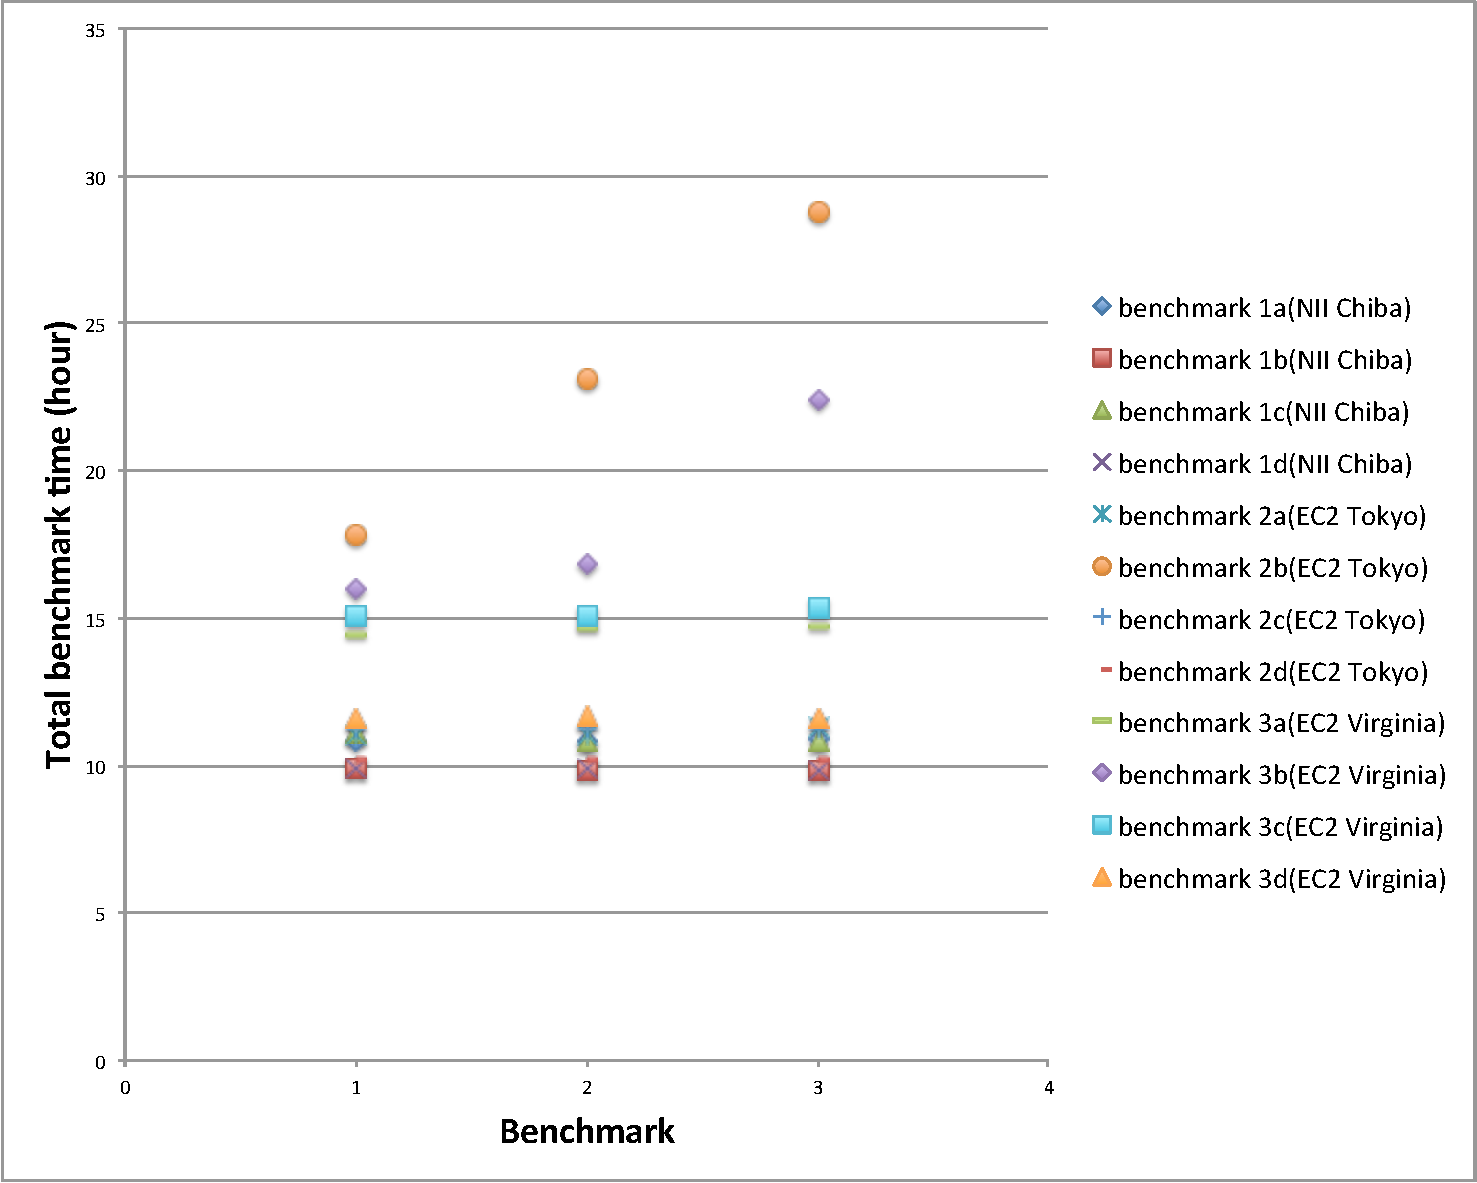
\includegraphics[width=0.8\textwidth,natwidth=900,natheight=600]{2_Total_benchmark_time.pdf}
  \end{center}
  \caption{Total benchmark time}
  \label{t_bench_t}
\end{figure}

\subsection{Docker image migration time}
\cref{t_bench_t} shows the total benchmark time for all benchmark settings. The benchmark time consists of the transfer times for all images presented in \cref{bench_img_l}.
We repeatedly ran the experiment for each benchmark setting for three times.
We can find that the results of benchmark settings 2b and 3b are quite unstable when we run the Docker registry 2.0.1 on the EC2 nodes, while the results under other settings present indistinguishable total benchmark time among three repeated benchmarks.
This irrational phenomenon will be analyzed in detail later and we can get some interesting findings if we ignore it temporally.

\begin{figure}[ht]
  \begin{center}
  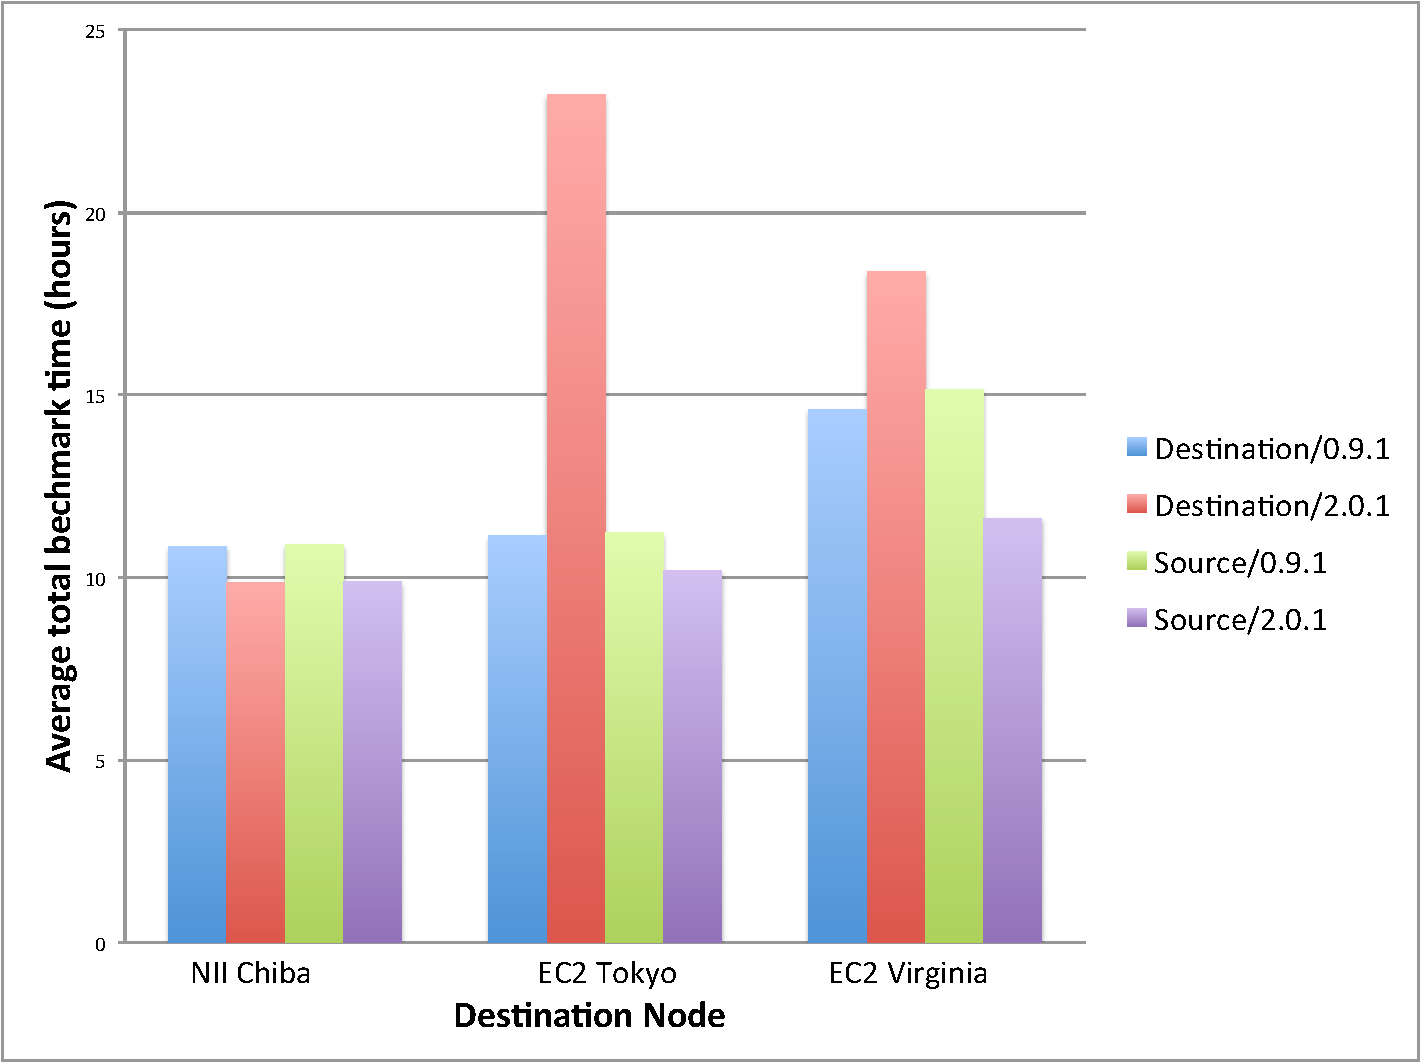
\includegraphics[width=0.8\textwidth,natwidth=1000,natheight=800]{3_Average_total_benchmark_time.pdf}
  \end{center}
  \caption{Average total benchmark time}
  \label{avg_bench_time}
\end{figure}


\cref{avg_bench_time} presents the average of three repeated benchmarks categorized by the destination node.
It shows that the performance of transferring Docker images from NII Tokyo Node to NII Chiba Nodes is slightly better than to EC2 Nodes, while transferring Docker images to EC2 Virginia node shows the worst performance because it locates in US.
We measured the latency and bandwidth between the source node and the destination nodes using ping and iperf \cite{iperf2015}, respectively.
\cref{lat_band} shows the latency and the bandwidth between NII Tokyo Node and three destination nodes. We can see that the benchmark results are in line with the bandwidth.

\begin{table}[ht]
  \begin{tabular}{|c|c|c|c|}
    \hline
    Destination & NII Chiba      & EC2 Tokyo    & EC2 Virginia \\
    \hline
    Latency     & 4.700ms        & 2.363ms      & 197.435ms \\
    \hline
    Bandwidth   & 941Mb/s        & 921.67Mb/s   & 53.48Mb/s \\
    \hline
  \end{tabular}
  \caption{Latency and bandwidth result}
  \label{lat_band}
\end{table}


\begin{figure}[ht]
  \begin{center}
  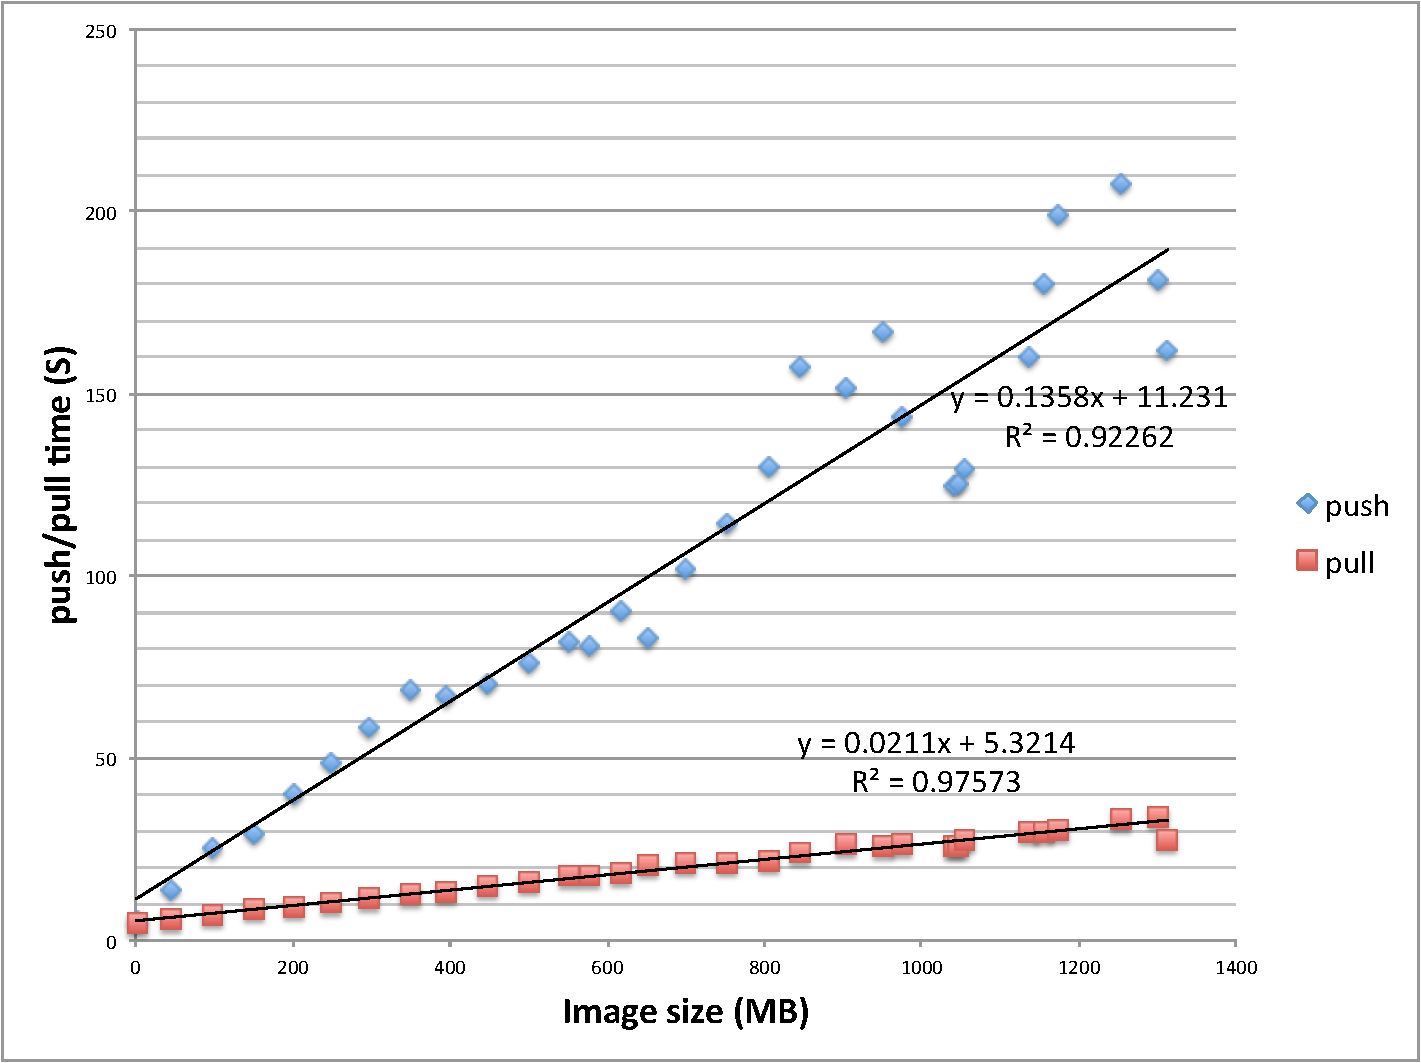
\includegraphics[width=0.8\textwidth,natwidth=1000,natheight=800]{4_push_and_pull_time.pdf}
  \end{center}
  \caption{Push and pull time}
  \label{ppt}
\end{figure}

The transfer time of a Docker image consists of the time to push the image to the Docker registry and the time to pull the image from the Docker registry.
\cref{ppt} shows the pull and push time of 31 images with different sizes in the benchmark 1a1.
In fact, all benchmarks share common features, except for the linear regression functions are different.
According to \cref{ppt}, both push and pull time present strong linear relationship with the image size.
We expected that push and pull time should be related to the number of layers and the layer size.
However, we do not see any significant evidence. Therefore, the linear regression function is enough to model the push and pull time.
\cref{ppt} includes the linear regression model derived from the results. Another obvious phenomenon in the figure is that the pull outperforms push and other benchmarks also show the same result.
The performance difference of compression and decompression processes should be the primary reason behind it.
When we push a Docker image, each layer of the image is compressed into a tar.gz file.
And the tar.gz file is decompressed when we pull the image.

\subsection{Docker registry versions and locations}

\begin{table}[ht]
  \begin{tabular}{|c|c|c|c|c|}
\hline
Registry location & Registry version & NII Cloud & EC2 Tokyo & EC2 Virginia \\
\hline
Destination       & 0.9.1            & 25.9\%     & 35.3\% & 35.2\% \\
\hline
Destination       & 2.0.1            & 0         & 7.4\%  & 7.0\% \\
\hline
Source            &  0.9.1           & 31.9\%     & 38.2\% & 40.7\% \\
\hline
Source            &  2.0.1           & 0         & 6.5\%  & 6.5\% \\
\hline
  \end{tabular}
  \caption{Docker registry fail rate}
  \label{reg_fail_rate}
\end{table}


The Docker registry 0.9.1 is written by python while the Docker registry 2.0.1 is implemented in Go language.
Thus, they are quite different. We can find that the Docker registry 2.0.1 shows better performance than the Docker registry 0.9.1 from \cref{t_bench_t} and \cref{avg_bench_time}.
In addition, the Docker registry 0.9.1 is easier to fail than the Docker registry 2.0.1.
\cref{reg_fail_rate} shows the Docker registry fail rate of all benchmarks. Therefore, the Docker registry 2.0.1 should be a better choice for Docker users considering performance and reliability.

When we run the Docker registry in a Docker container, we can run the registry container on the source node (NII Tokyo Node) or the destination node (NII Chiba, EC2 Tokyo or EC2 Virginia Nodes).
\cref{t_bench_t} indicates that the location of the Docker registry does not affect the transfer performance except the results of the benchmark settings 2b and 3b.

\subsection{Discussion about instability}

\begin{figure}[ht]
  \begin{center}
  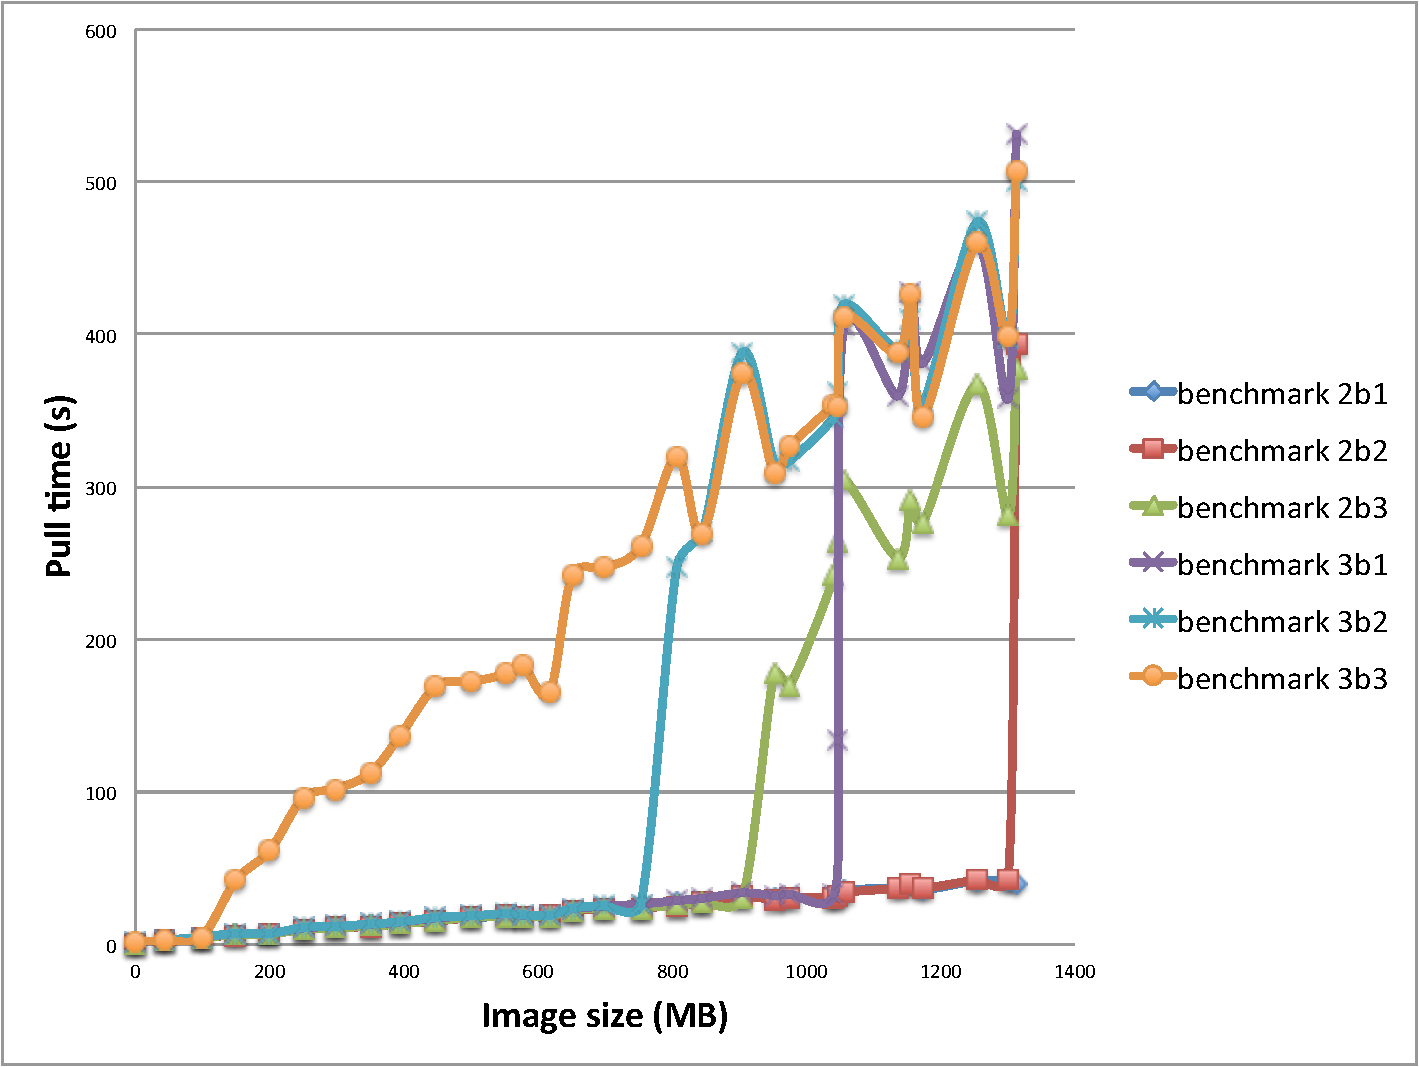
\includegraphics[width=0.8\textwidth,natwidth=1100,natheight=500]{5_pull_time_of_running_docker_registry_2.0.1_on_EC2_nodes.pdf}
  \end{center}
  \caption{Pull time of running registry 2.0.1 on EC2 Nodes}
  \label{pull_time}
\end{figure}

As we mentioned above, the benchmark results are quite unstable when we ran the Docker registry 2.0.1 on EC2 nodes, which are destination nodes.
Our detailed analysis indicates that the instability is caused by the sudden degradation of pull performance.
\cref{pull_time} shows pull time for the benchmark setting 2b and 3b, where we repeatedly run the benchmark three times for each.
For example, benchmark 2b1 indicates the results of the first run under the setting 2b.
According to the results of other benchmarks, the pull time shows strong linear relationship with the Docker image size.
However, only the pull time of benchmark 2b1 fit in the linear relationship with image size.
For others, the pull time increased suddenly from some point as we can see in \cref{pull_time}.
In the benchmark setting, the network performance between the source and the destination does not affect the pull performance, because the Docker registry runs in the destination node.
Thus, we guess that the implementation of the Docker registry 2.0.1 or the EC2 instance is related to the performance degradation.
We leave the further investigation for future work.


\section{Conclusion}
In the era of big data and cloud computing, how to utilize clouds to perform big data analysis is becoming a practical issue. The rise of container technology such as Docker bring a new opportunity for deploying big data application in clouds, because it helps us simplify tedious software configuration process and provides great portability across multiple clouds. However, the resource selection problem challenges users to maximize performance.


In this paper, we evaluated Docker image transfer time as the first step to tackle the optimal resource selection problem. The results show that the Docker image transfer time, including push and pull time, increases linearly with the image size and shows negligible relationship with the number of image layers or the layer size. We also find that the Docker registry 2.0.1 outperforms the registry 0.9.1 and it exhibits better reliability. Thus, the Docker registry 2.01 should be a better choice for Docker users.


In the future, we intend to investigate the performance instability of running Docker registry 2.0.1 on EC2 nodes. This can help us understand the Docker image transfer performance better. Furthermore, we plan to build the mathematical model of Docker image transfer time by running more benchmarks.


\bibliographystyle{sieicej}
\bibliography{myrefs.bib}


% \begin{biography}
% \profile{}{}{}
% \profile{会員種別}{名前}{紹介文}% 顔写真あり
% \profile*{会員種別}{名前}{紹介%文}% 顔写真なし
% \end{biography}

\end{document}

